\documentclass[12pt]{article}

% Packages
\usepackage{amsmath} % For align* environment
\usepackage{enumitem} % For itemize/enumerate customization (optional, but keeps options from beamer)
\usepackage{booktabs} % For tables (not strictly used with verbatim, but good practice)
\usepackage{tikz} % For TikZ diagrams (if any are implicitly generated)
\usepackage{tikz-qtree} % For qtrees (if any are implicitly generated)
\usepackage{xcolor} % For colors
\usepackage{graphicx} % For including figures
\usepackage{listings} % For code snippets
\usepackage[margin=1in]{geometry}
% Define graphicspath relative to the TeX file location
\graphicspath{{figures/}} % Match python FIG_DIR

% Code listing style (similar to previous, adjust colors/style as desired)
\definecolor{codegreen}{rgb}{0,0.6,0}
\definecolor{codegray}{rgb}{0.5,0.5,0.5}
\definecolor{codepurple}{rgb}{0.58,0,0.82}
\definecolor{backcolour}{rgb}{0.98,0.98,0.98} % Light background for code

\lstdefinestyle{mystyle}{
    backgroundcolor=\color{backcolour},
    commentstyle=\itshape\color{codegreen}, % Italic comments
    keywordstyle=\bfseries\color{blue}, % Bold keywords
    numberstyle=\tiny\color{codegray},
    stringstyle=\color{codepurple},
    basicstyle=\ttfamily\footnotesize,
    breakatwhitespace=false,
    breaklines=true,
    captionpos=b,
    keepspaces=true,
    numbers=left,
    numbersep=5pt,
    showspaces=false,
    showstringspaces=false,
    showtabs=false,
    tabsize=2,
    language=Python
}
\lstset{style=mystyle}

% Custom symbols (redefined from beamer preamble)
\DeclareMathOperator{\Normal}{Normal}
\DeclareMathOperator{\HalfNormal}{HalfNormal}
\DeclareMathOperator{\Binomial}{Binomial}
\newcommand{\Phicdf}{\Phi} % Use \Phi for Normal CDF

% Title page info
\title{Identifiability}
\author{Joachim Vandekerckhove}
\date{Spring 2025}

\begin{document}

\section*{Identifiability}

In statistical and cognitive modeling, particularly when we deal with complex or custom models, a crucial concept is \emph{identifiability}. A model is considered \emph{non-identifiable} if there exist different combinations of the model's parameters that always produce exactly the same predictions. In the context of likelihood-based models, this implies that distinct parameter sets yield identical likelihood values for any potential observed data.  As a result no amount of observed data can distinguish between these parameter constellations. This makes it impossible to infer parameters from data -- the data do not provide enough information to uniquely determine the true underlying parameters.

There are nuances to different kinds of non-identifiability, but certainly the most problematic type is \textbf{structural non-identifiability}, which is not due to insufficient data or poor experimental design, but is inherent in the mathematical structure of the model's equations themselves.

Fitting a non-identifiable model using MCMC methods typically results in several observable difficulties:
\begin{itemize}
    \item Poor MCMC convergence, characterized by high values of the $\hat{R}$ convergence statistic (much greater than 1) and low Effective Sample Sizes (ESS).
    \item Posterior distributions that look unstable, that drift, or take on unusual shapes.
    \item Strong correlations among the parameters affected by the non-identifiability in the posterior samples.
\end{itemize}

Those three symptoms are visible -- but the fourth symptom is the problem: unidentified models are not suitable for statistical inference.  You cannot estimate their parameters and you cannot draw conclusions about them.  Avoiding or addressing non-identifiability is a necessary step for valid model-based inference.


\subsection*{Illustrative Example: A Hierarchical Signal Detection Theory Model}

Consider a hierarchical Signal Detection Theory (SDT) model as an example. Consider a simple SDT model that predicts counts of Hits ($H_{ip}$) and False Alarms ($F_{ip}$) for person $p$ in condition $i$.

The data are modeled via a \textbf{likelihood} derived from Binomial distributions, where the success probabilities are determined by SDT parameters: sensitivity ($d'_{ip}$) and criterion ($c_p$), along with trial counts ($n_s, n_n$).  Jointly, these equations (which we have covered many times) can be used to compute the likelihood of the data given the parameters.  We can write this abstractly as:
\begin{align*}
  \left(H_{ip}, F_{ip}\right) &\sim SDT\left(d'_{ip}, c_p, n_s, n_n\right)
\end{align*}

Within a \textbf{hierarchical signal detection theory (HSDT) model}, the parameters $d'_{ip}$ and $c_p$ have some sort of structure.  Let's suppose a very reasonable HSDT model, in which $d'_{ip}$ is defined as the sum of a person-specific intercept $\alpha_p$ and a condition-specific effect $\gamma_i$:
\begin{align*}
  d'_{ip} &= \alpha_p + \gamma_i
\end{align*}
The condition effect $\gamma_i$ is specified linearly based on a condition-level predictor:
\begin{align*}
  \gamma_i &= \zeta_0 + \zeta_1 \cdot \text{predictor}_i \quad &\text{(Condition effect on } d')
\end{align*}
$\zeta_0$ functions as the intercept for the condition effect and $\zeta_1$ is the slope (i.e., effect size) of the condition effect.

The person intercept $\alpha_p$ is drawn from a group-level distribution to allow pooling of information across people:
\begin{align*}
  \alpha_p &\sim \Normal(\mu_\alpha, \sigma^2_\alpha) \quad &\text{(Person sensitivity intercept)}
\end{align*}
The person criterion $c_p$ is also modeled hierarchically (but less relevant here):
\begin{align*}
  c_p &\sim \Normal(\mu_c, \sigma^2_c) \quad &\text{(Person criterion)}
\end{align*}
The identifiability issue in this formulation is concentrated within the specification of $d'_{ip}$.


\subsection*{Analysis of Non-Identifiability}

The source of the non-identifiability in this model is revealed by substituting the definition of $\gamma_i$ into the equation for $d'_{ip}$:
\begin{align*}
  d'_{ip} &= \alpha_p + \gamma_i \\
         &= \alpha_p + (\zeta_0 + \zeta_1 \cdot \text{predictor}_i) \\
         &= (\alpha_p + \zeta_0) + \zeta_1 \cdot \text{predictor}_i
\end{align*}
The parameter $d'_{ip}$ depends on the sum of the person intercept $\alpha_p$ and the condition effect intercept $\zeta_0$, in addition to the term involving $\zeta_1$ and the predictor.  A jargon-y way of describing this setup is that $d'_{ip}$ has two intercepts (or rather, two parameters that each act as an intercept).

Since the model likelihood depends on $d'_{ip}$ and $c_p$, it is determined by the value of the sum $(\alpha_p + \zeta_0)$ and the term $\zeta_1 \cdot \text{predictor}_i$.

We can now consider two distinct parameter sets. Let one set contain $(\alpha_p, \zeta_0)$ and another contain $(\tilde{\alpha}_p, \tilde{\zeta}_0)$, where $\tilde{\alpha}_p = \alpha_p - C$ and $\tilde{\zeta}_0 = \zeta_0 + C$ for an arbitrary constant $C$. The sum for the second set is:
\[ \tilde{\alpha}_p + \tilde{\zeta}_0 = (\alpha_p - C) + (\zeta_0 + C) = \alpha_p + \zeta_0 \]

As is hopefully obvious, any constant $C$ could be added to $\zeta_0$ and subtracted from $\alpha_p$ without altering their sum. Consequently, the calculated value of $d'_{ip}$ remains unchanged. As $d'_{ip}$ (and an identifiable $c_p$) determines the likelihood, these distinct parameter combinations yield identical likelihood distributions, always.  In other words, the individual values of $\alpha_p$ and $\zeta_0$ are arbitrary (even though their sum is not).

$\alpha_p$ and $\zeta_0$ are said to be confounded additively. At the group level, this manifests as an inability to distinguish between the mean person sensitivity $\mu_\alpha$ and the condition intercept $\zeta_0$. The model structure permits trade-offs between these parameters while maintaining the same likelihood. This constitutes \emph{structural non-identifiability}.


\subsection*{Common MCMC Symptoms}

MCMC diagnostics can help us identify non-identifiability.  When a non-identified model is fit using MCMC methods, several diagnostic indicators should raise red flags:

\begin{itemize}[label=--, itemsep=1ex]
    \item \textbf{Poor Convergence} for the parameters involved in the confounding (e.g., $\mu_\alpha$ and $\zeta_0$). This is shown by high $\hat{R}$ values and low Effective Sample Sizes (ESS).
    \item \textbf{Wandering Trace Plots}. The MCMC chains for the confounded parameters may exhibit poor mixing and fail to stabilize, often appearing to explore a `ridge' of high likelihood.
    \item \textbf{Strong Posterior Correlation}. Visual analysis of the joint posterior distribution (or pairwise plots) of the confounded parameters may show a dependency. In this additive case, a negative linear correlation between $\mu_\alpha$ and $\zeta_0$ is expected, but in general the relationship need not be linear, and it may even involve many parameters. (In fact, in the example scenario, every $alpha_p$ is also involved.)
    \item \textbf{Sampling Difficulties}. Numerical stability issues may arise, potentially leading to sampler warnings such as divergences.
\end{itemize}
These observations collectively signal the presence of non-identifiability.

\subsection*{PyMC Implementation of the Non-Identified Model}

The following PyMC code snippet illustrates the parameter definitions that lead to the non-identifiability in the hierarchical SDT model. (Find the full code in the GitHub repository, \texttt{0-introduction/src/sdt/sdt\_identifiability.py}.)

\begin{lstlisting}[label=lst:nonid_sdt_code, caption={PyMC code snippet for the non-identified SDT model parameters.}]
# Uninformative priors for Sensitivity (d') parameters
mu_alpha = pm.Normal("mu_alpha", mu=0.0, sigma=1.0e9) # << Part 1
sigma_alpha = pm.HalfNormal("sigma_alpha", sigma=1.0e9)
zeta0 = pm.Normal("zeta0", mu=0.0, sigma=1.0e9)       # << Part 2
zeta1 = pm.Normal("zeta1", mu=0.0, sigma=1.0e9)

# Person sensitivity intercepts (drawn from mu_alpha)
alpha_p = pm.Normal("alpha_p", mu=mu_alpha, sigma=sigma_alpha)

# Calculate gamma_i (Condition effect on d')
# (Assuming 'cond_pred_data' is available elsewhere)
gamma_i = zeta0 + zeta1 * cond_pred_data

# Calculate d' using alpha_p and gamma_i
d_ip = pm.Deterministic("d_ip", alpha_p[...] + gamma_i) # << Part 3

# ... SDT likelihood calculations using d_ip and c_p ...
\end{lstlisting}
The inclusion of `mu\_alpha` (Part 1, mean of person intercepts) and `zeta0` (Part 2, intercept of condition effects), combined with their additive contribution to `d\_ip` (Part 3 via `alpha\_p` and `gamma\_i`), introduces a structural redundancy.

\subsection*{Diagnosis Method 1: Trace Plots}

Evaluation of MCMC trace plots provides a visual diagnostic for convergence and mixing issues. Using `arviz.plot\_trace()`, focused on parameters such as `mu\_alpha` and `zeta0`, is standard practice.

When reviewing trace plots, pay attention to:
\begin{itemize}[label=--, itemsep=1ex]
    \item Indications of poor mixing among the distinct chains for `mu\_alpha` and `zeta0` -- the chains should look like they are drawing samples from a stationary distribution and not wandering up and down.  A well-mixed trace plot is sometimes described as a `fat, hairy caterpillar'.
    \item Evidence of chains exploring separate regions or failing to converge to a common stationary distribution.  All chains should converge to the same region of the parameter space.
    \item Cross-check visual findings with high $\hat{R}$ values reported in the MCMC summary.
\end{itemize}
Figure \ref{fig:nonid_trace} presents trace plots from a fit of the non-identified model. Here we see the expected poor mixing and wandering for the confounded parameters. By contrast, Figure \ref{fig:id_trace} shows well-behaved traces from an identified version of the model.

\begin{figure}[tbhp]
    \centering
    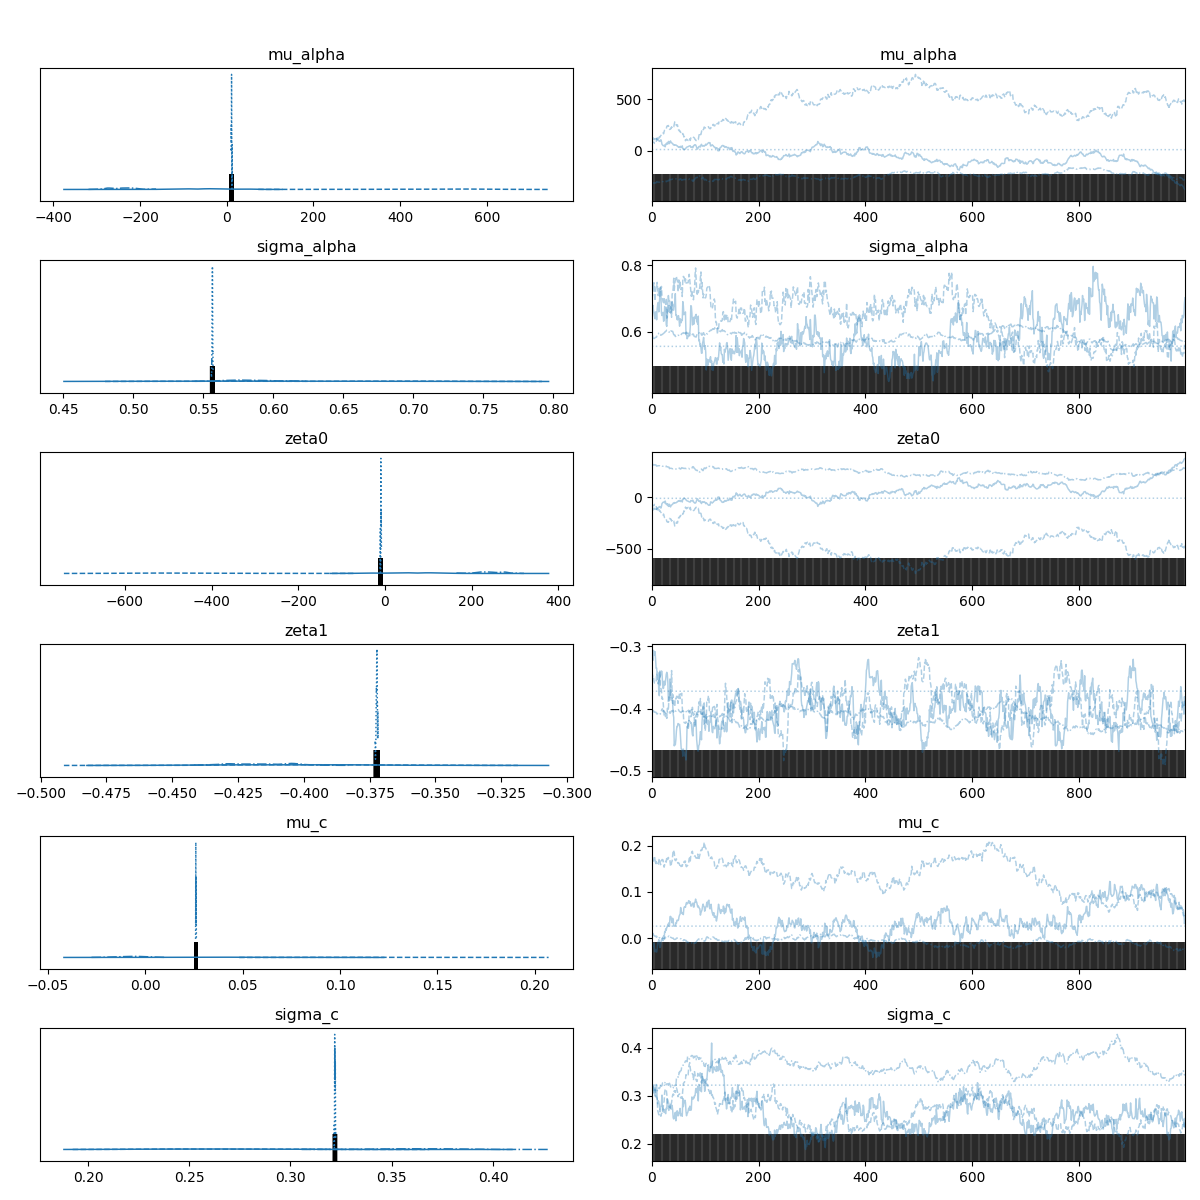
\includegraphics[width=\linewidth]{nonid_sdt_trace.png}
    \caption{Trace plots for key parameters from the non-identified SDT model. Poor mixing and wandering chains are $\mu_\alpha$ and $\zeta_0$'s lot.}
    \label{fig:nonid_trace}
\end{figure}

\begin{figure}[tbhp]
    \centering
    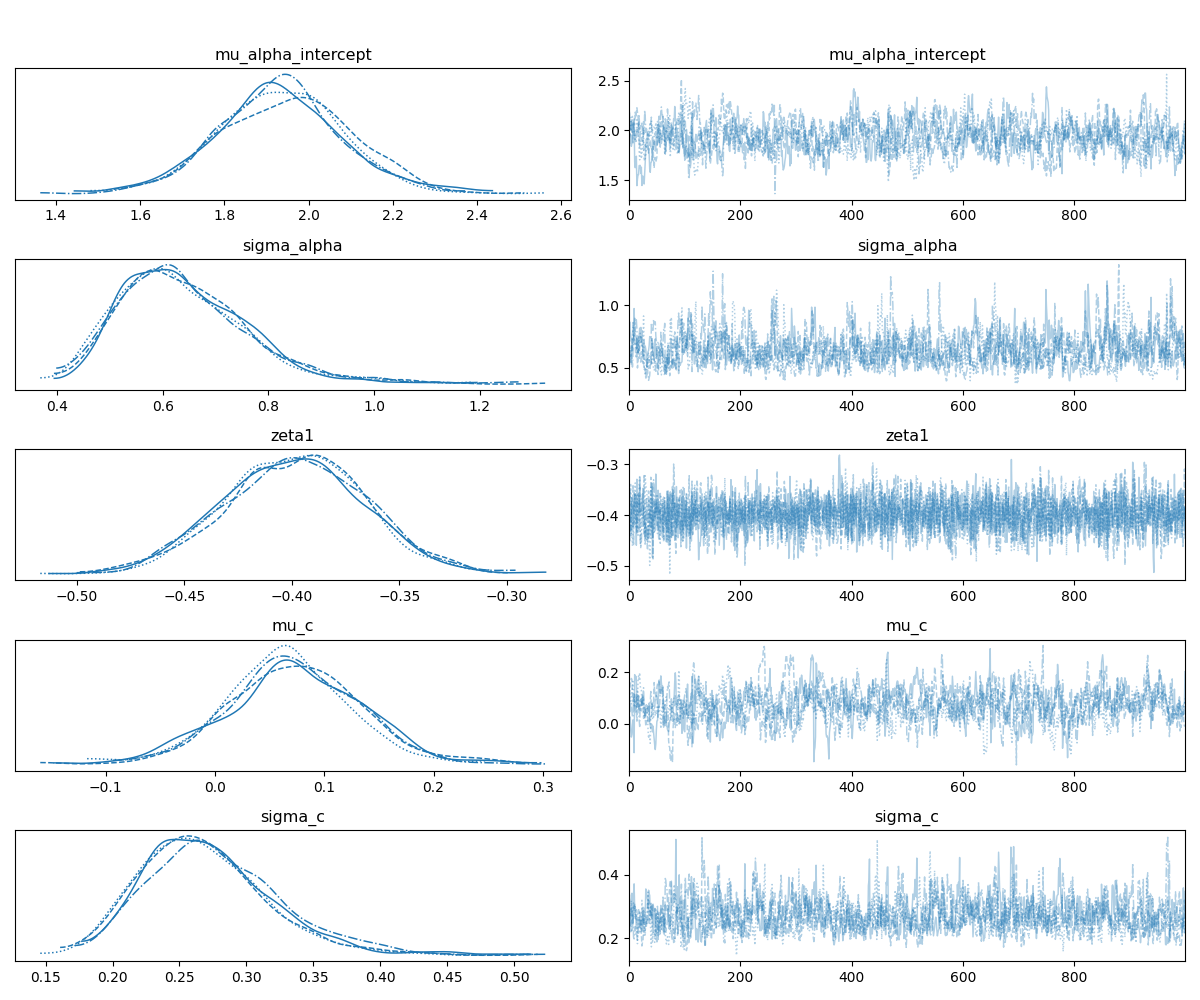
\includegraphics[width=\linewidth]{id_sdt_trace.png}
    \caption{Trace plots for key parameters from the identified SDT model. Chains show good mixing and convergence.}
    \label{fig:id_trace}
\end{figure}


\subsection*{MCMC Output Summary}

Quantitative assessment of MCMC performance is provided by the summary table. The summary for the non-identified model looks like this:

\footnotesize
\begin{verbatim}
    --- Non-Identified SDT Model Summary ---
             mean       sd   hdi_3%  hdi_97%  mcse_mean  mcse_sd  ess_bulk  ess_tail  r_hat
mu_alpha   40.779  268.443 -304.985  570.827    128.271   70.199       5.0      17.0   2.70
zeta0     -38.809  268.503 -569.032  307.068    128.298   70.209       5.0      17.0   2.70
zeta1      -0.397    0.028   -0.446   -0.350      0.008    0.001      15.0     180.0   1.22
mu_c        0.048    0.058   -0.020    0.173      0.027    0.014       5.0      26.0   2.35
Sampling 4 chains for 1_500 tune and 1_000 draw iterations (6_000 + 4_000 draws total) took 379s.
There were 1000 divergences after tuning. Increase `target_accept` or reparameterize.
\end{verbatim}
\normalsize

The high $\hat{R}$ values (2.70) and extremely low ESS (5.0) for `mu\_alpha` and `zeta0` indicate poor convergence. Seeing 1000 divergences is also a red flag (ideally, there are none).

For comparison, the summary from the identified model below indicates successful convergence, with $\hat{R}$ values near 1.0 and substantially higher ESS for all parameters, including the newly named `mu\_alpha\_intercept`.

\footnotesize
\begin{verbatim}
--- Identified SDT Model Summary ---
               mean       sd   hdi_3%  hdi_97%  mcse_mean  mcse_sd  ess_bulk  ess_tail  r_hat
mu_alpha_int  1.936    0.149    1.659    2.221      0.008    0.004     380.0     598.0   1.01
zeta1        -0.398    0.033   -0.463   -0.341      0.001    0.000    3558.0    3080.0   1.00
mu_c          0.072    0.062   -0.046    0.186      0.003    0.002     426.0     735.0   1.01
Sampling 4 chains for 1_500 tune and 1_000 draw iterations (6_000 + 4_000 draws total) took 12s.
\end{verbatim}
\normalsize

\subsection*{Diagnosis Method 2: Pair Plots}

Pair plots show the joint posterior distributions of pairs of parameters. This is a diagnostic for (possibly non-linear) correlations indicative of identifiability issues. The `arviz.plot\_pair()` function, applied to `mu\_alpha` and `zeta0`, is useful here.

When examining pair plots for potentially confounded parameters, features to identify include:
\begin{itemize}[label=--, itemsep=1ex]
    \item A distinct correlation forming a ``ridge'' across the scatter plot of posterior samples.
    \item Specifically for this additive confounding, a \emph{negative, linear} correlation between `mu\_alpha` and `zeta0`.
    \item Marginal distributions along the diagonal that may appear unusually flat or poorly defined -- they will have excess variance compared the true posterior distributions.
\end{itemize}
Figure \ref{fig:nonid_pair} displays the pair plot for `mu\_alpha` and `zeta0` from the non-identified model --  a strong negative linear correlation is visible.

\begin{figure}[tbhp]
    \centering
    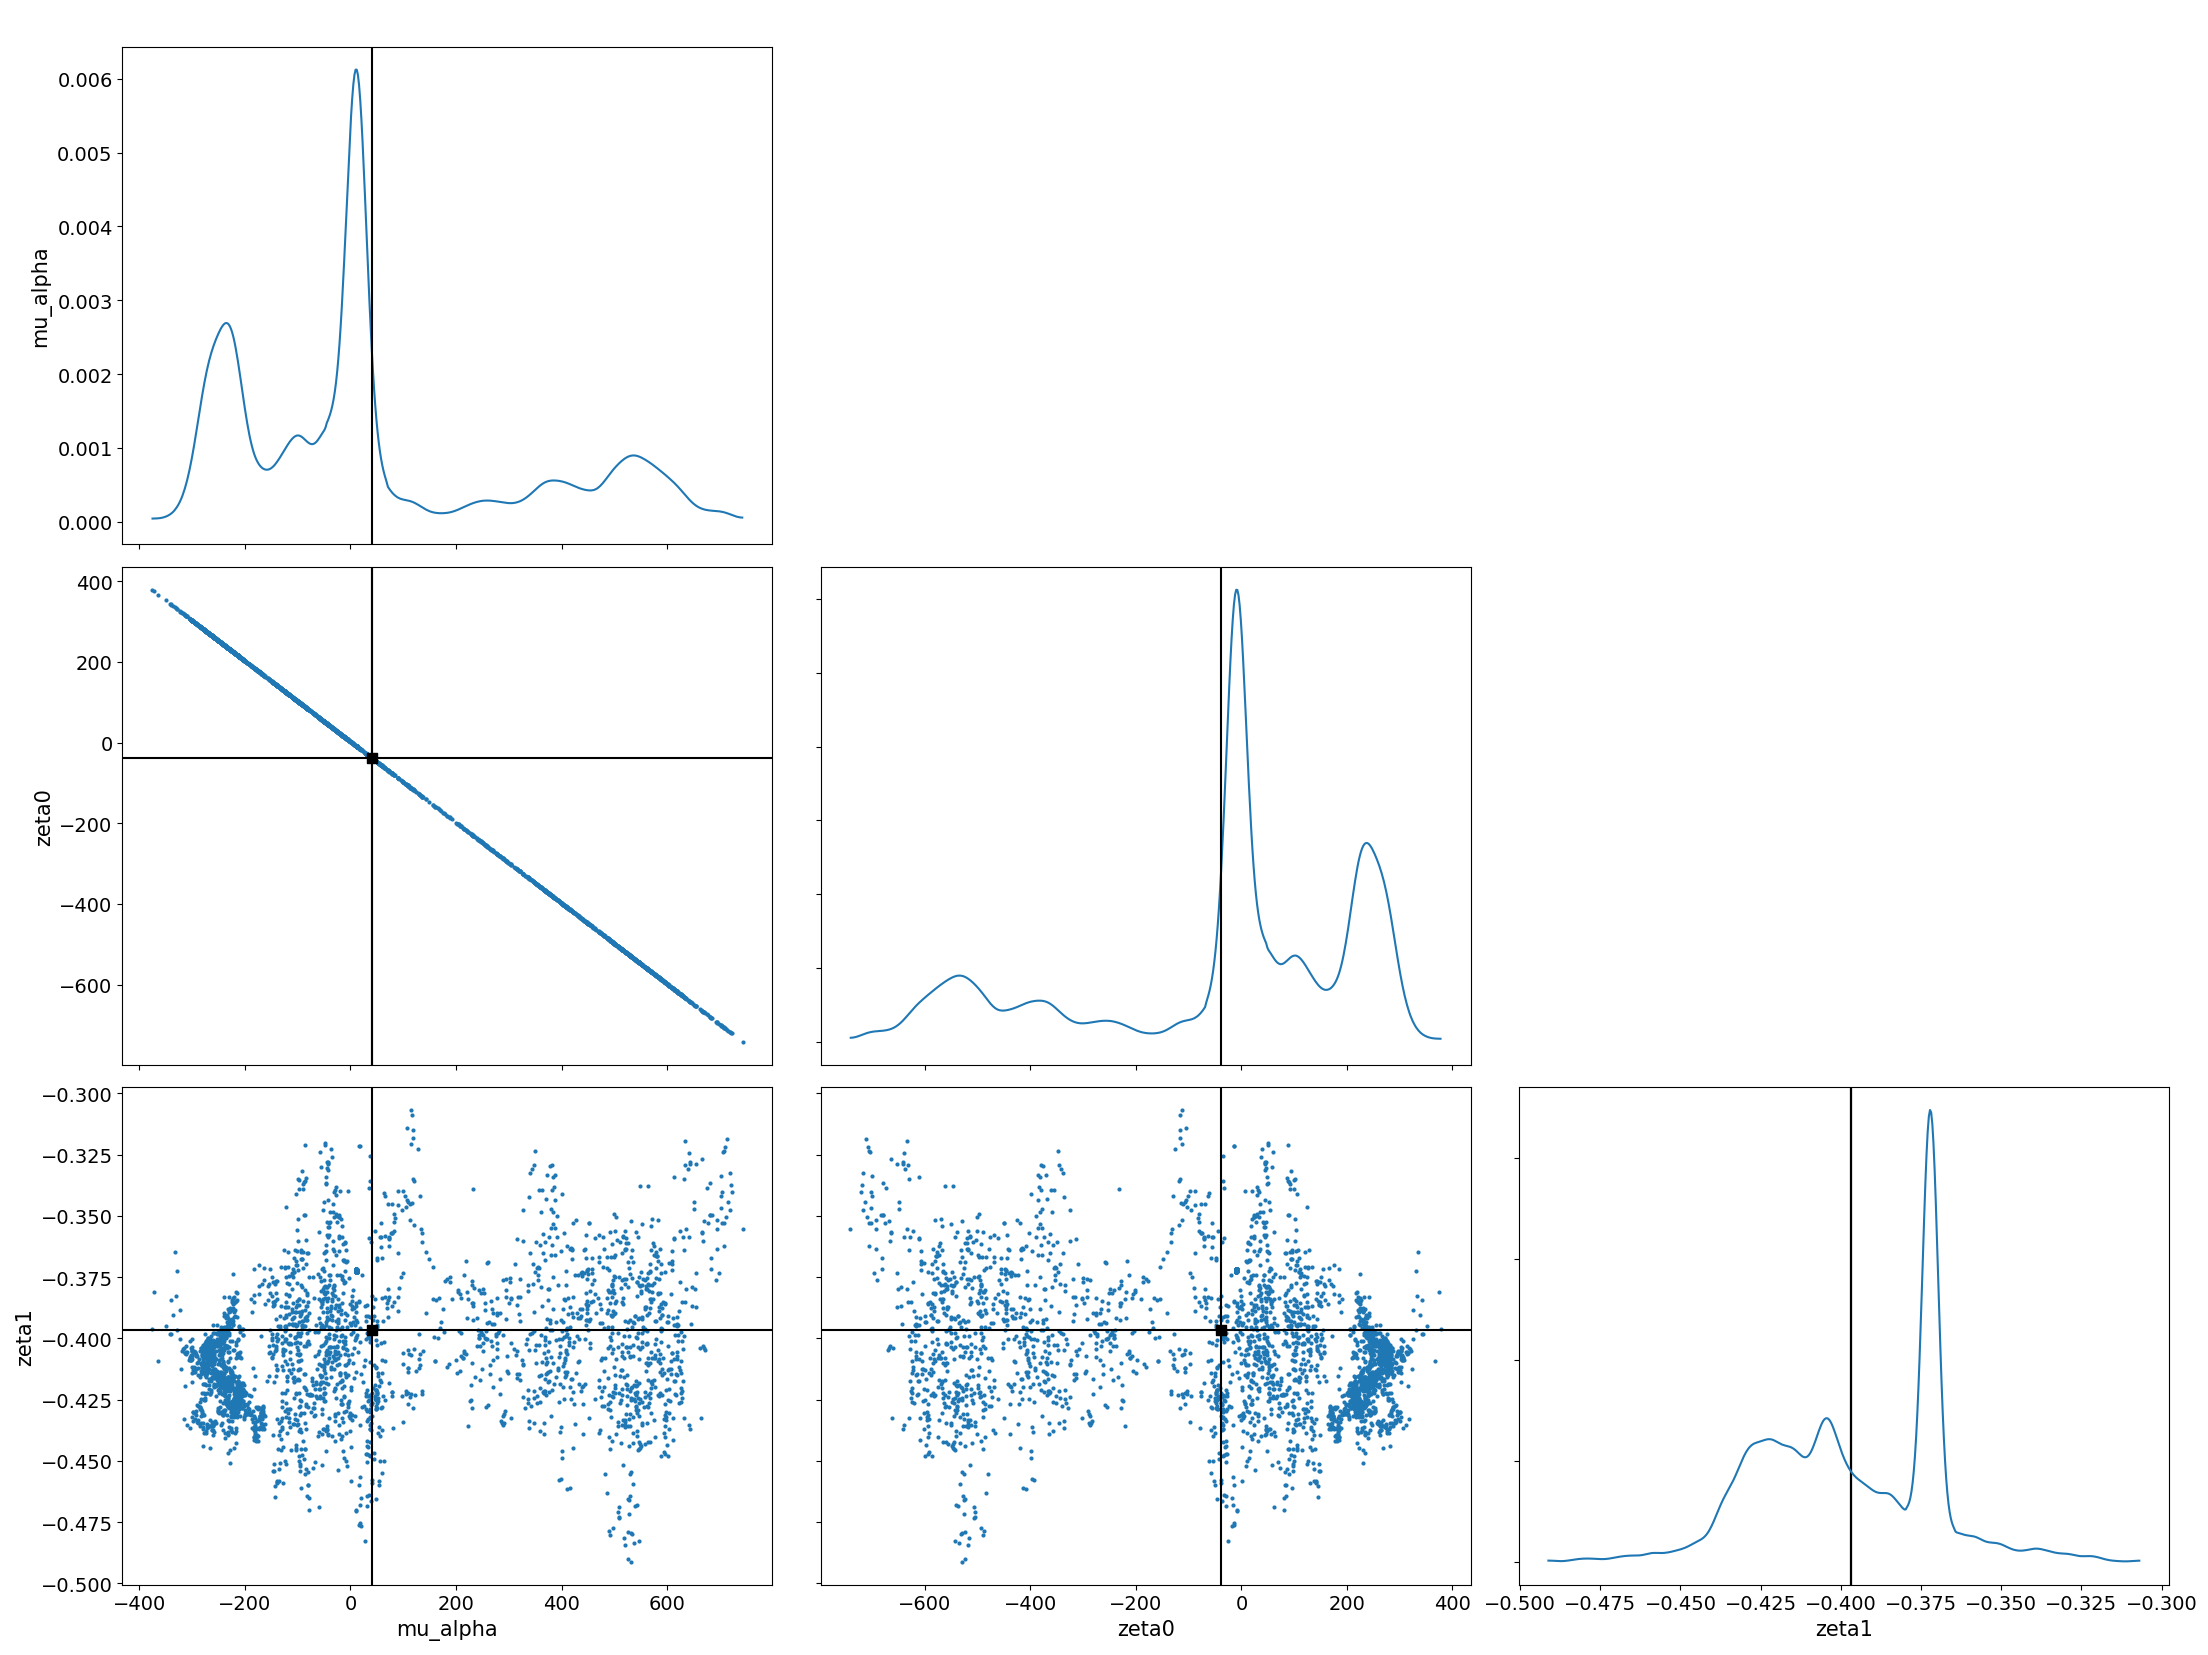
\includegraphics[width=\linewidth]{nonid_sdt_pair.png}
    \caption{Pair plot for $\mu_\alpha$ and $\zeta_0$ from the non-identified SDT model. A strong negative linear correlation indicates confounding, and the marginal posteriors on the diagonal have strange complex shapes.}
    \label{fig:nonid_pair}
\end{figure}


\subsection*{Strategies for Addressing Non-Identifiability}

Non-identifiability must be addressed to maintain valid statistical inference. Common strategies include:

\begin{enumerate}[label=\bf\alph*)]
    \item \textbf{Reparameterization (Preferred)}. This involves modifying the model's parameterization to remove the inherent redundancy. Methods include:
    \begin{itemize}[label=--, itemsep=0.5ex]
        \item Removing redundant parameters. In the example, removing $\zeta_0$ eliminates the additive confounding.
        \item Imposing sum-to-zero constraints on effects. This is an alternative method to resolve additive confounding but a little trickier to implement.
        \item Modeling effects as contrasts relative to a baseline condition. This implicitly removes a redundant intercept.
    \end{itemize}
    Reparameterization addresses the structural source of the issue.
    \item \textbf{Informative Priors}. Applying informative priors to confounded parameters can constrain the posterior and improve MCMC convergence diagnostics. However, this does not resolve the \emph{structural} non-identifiability. The resulting posterior distributions for the affected parameters will be heavily influenced by the chosen prior. That is not by itself a problem, but it is important not to forget that you may have made prior assumptions that drive your conclusions.
    \item \textbf{Exogenous Predictors}. Adding an exogenous predictor that is not confounded with the parameters of interest can resolve the non-identifiability. In the example, replacing the mean person intercept $\mu_\alpha$ with a function of a predictor variable (e.g., $\mu_\alpha = \zeta_1 \cdot \text{predictor}_i$) removes the confounding.
\end{enumerate}

Even though this is not the preferred approach, let's briefly look at the effect of informative priors.

\subsection*{Effect of Informative Priors}

Employing informative priors can lead to improved MCMC convergence statistics even in a structurally non-identified model. I sometimes call those models ``classically unidentified'' because they are not identified by the data, but they can be identified by the data and a Bayesian prior.

Using $\mu_\alpha \sim \Normal(0, 1.5)$ (a more informative prior than before) in the non-identified SDT model yields convergence statistics shown below.

\footnotesize
\begin{verbatim}
    --- Semi-Identified SDT Model Summary ---
    mean     sd  hdi_3%  hdi_97%  mcse_mean  mcse_sd  ess_bulk  ess_tail  r_hat
mu_alpha     1.301  0.827  -0.310    2.807      0.018    0.013    2023.0    2365.0   1.00
zeta0        0.629  0.825  -0.924    2.183      0.018    0.013    2002.0    2339.0   1.00
zeta1       -0.398  0.033  -0.459   -0.338      0.001    0.001    3915.0    2744.0   1.00
mu_c         0.067  0.064  -0.051    0.190      0.003    0.002     480.0     720.0   1.01
\end{verbatim}\normalsize

The $\hat{R}$ values are now near 1.00, and ESS values are considerably higher than in the standard non-identified fit. Trace plots (Figure \ref{fig:semiid_trace}) also appear more stable.  This looks almost good!

\begin{figure}[tbhp]
    \centering
    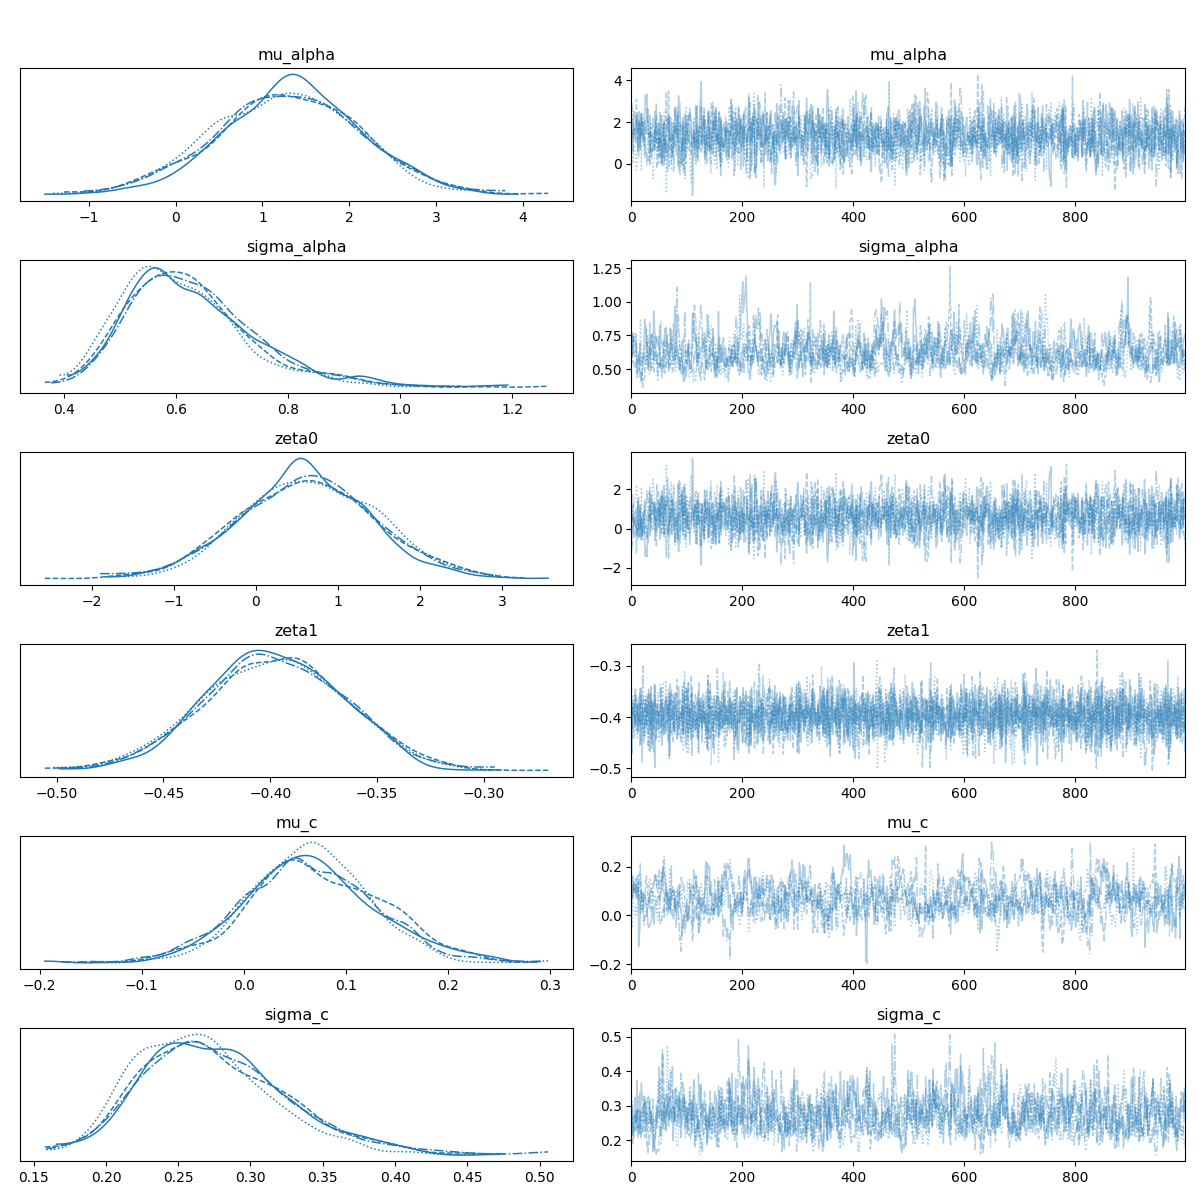
\includegraphics[width=\linewidth]{semiid_sdt_trace.png}
    \caption{Trace plots from the model with an informative prior on $\mu_\alpha$. Apparent convergence based on traces.}
    \label{fig:semiid_trace}
\end{figure}

However, the pair plot for `mu\_alpha` and `zeta0` (Figure \ref{fig:semiid_pair}) continues to show the underlying negative correlation ridge, even if it is a little jittered now. While the prior aided convergence, the structural confounding remains.

\begin{figure}[h!]
    \centering
    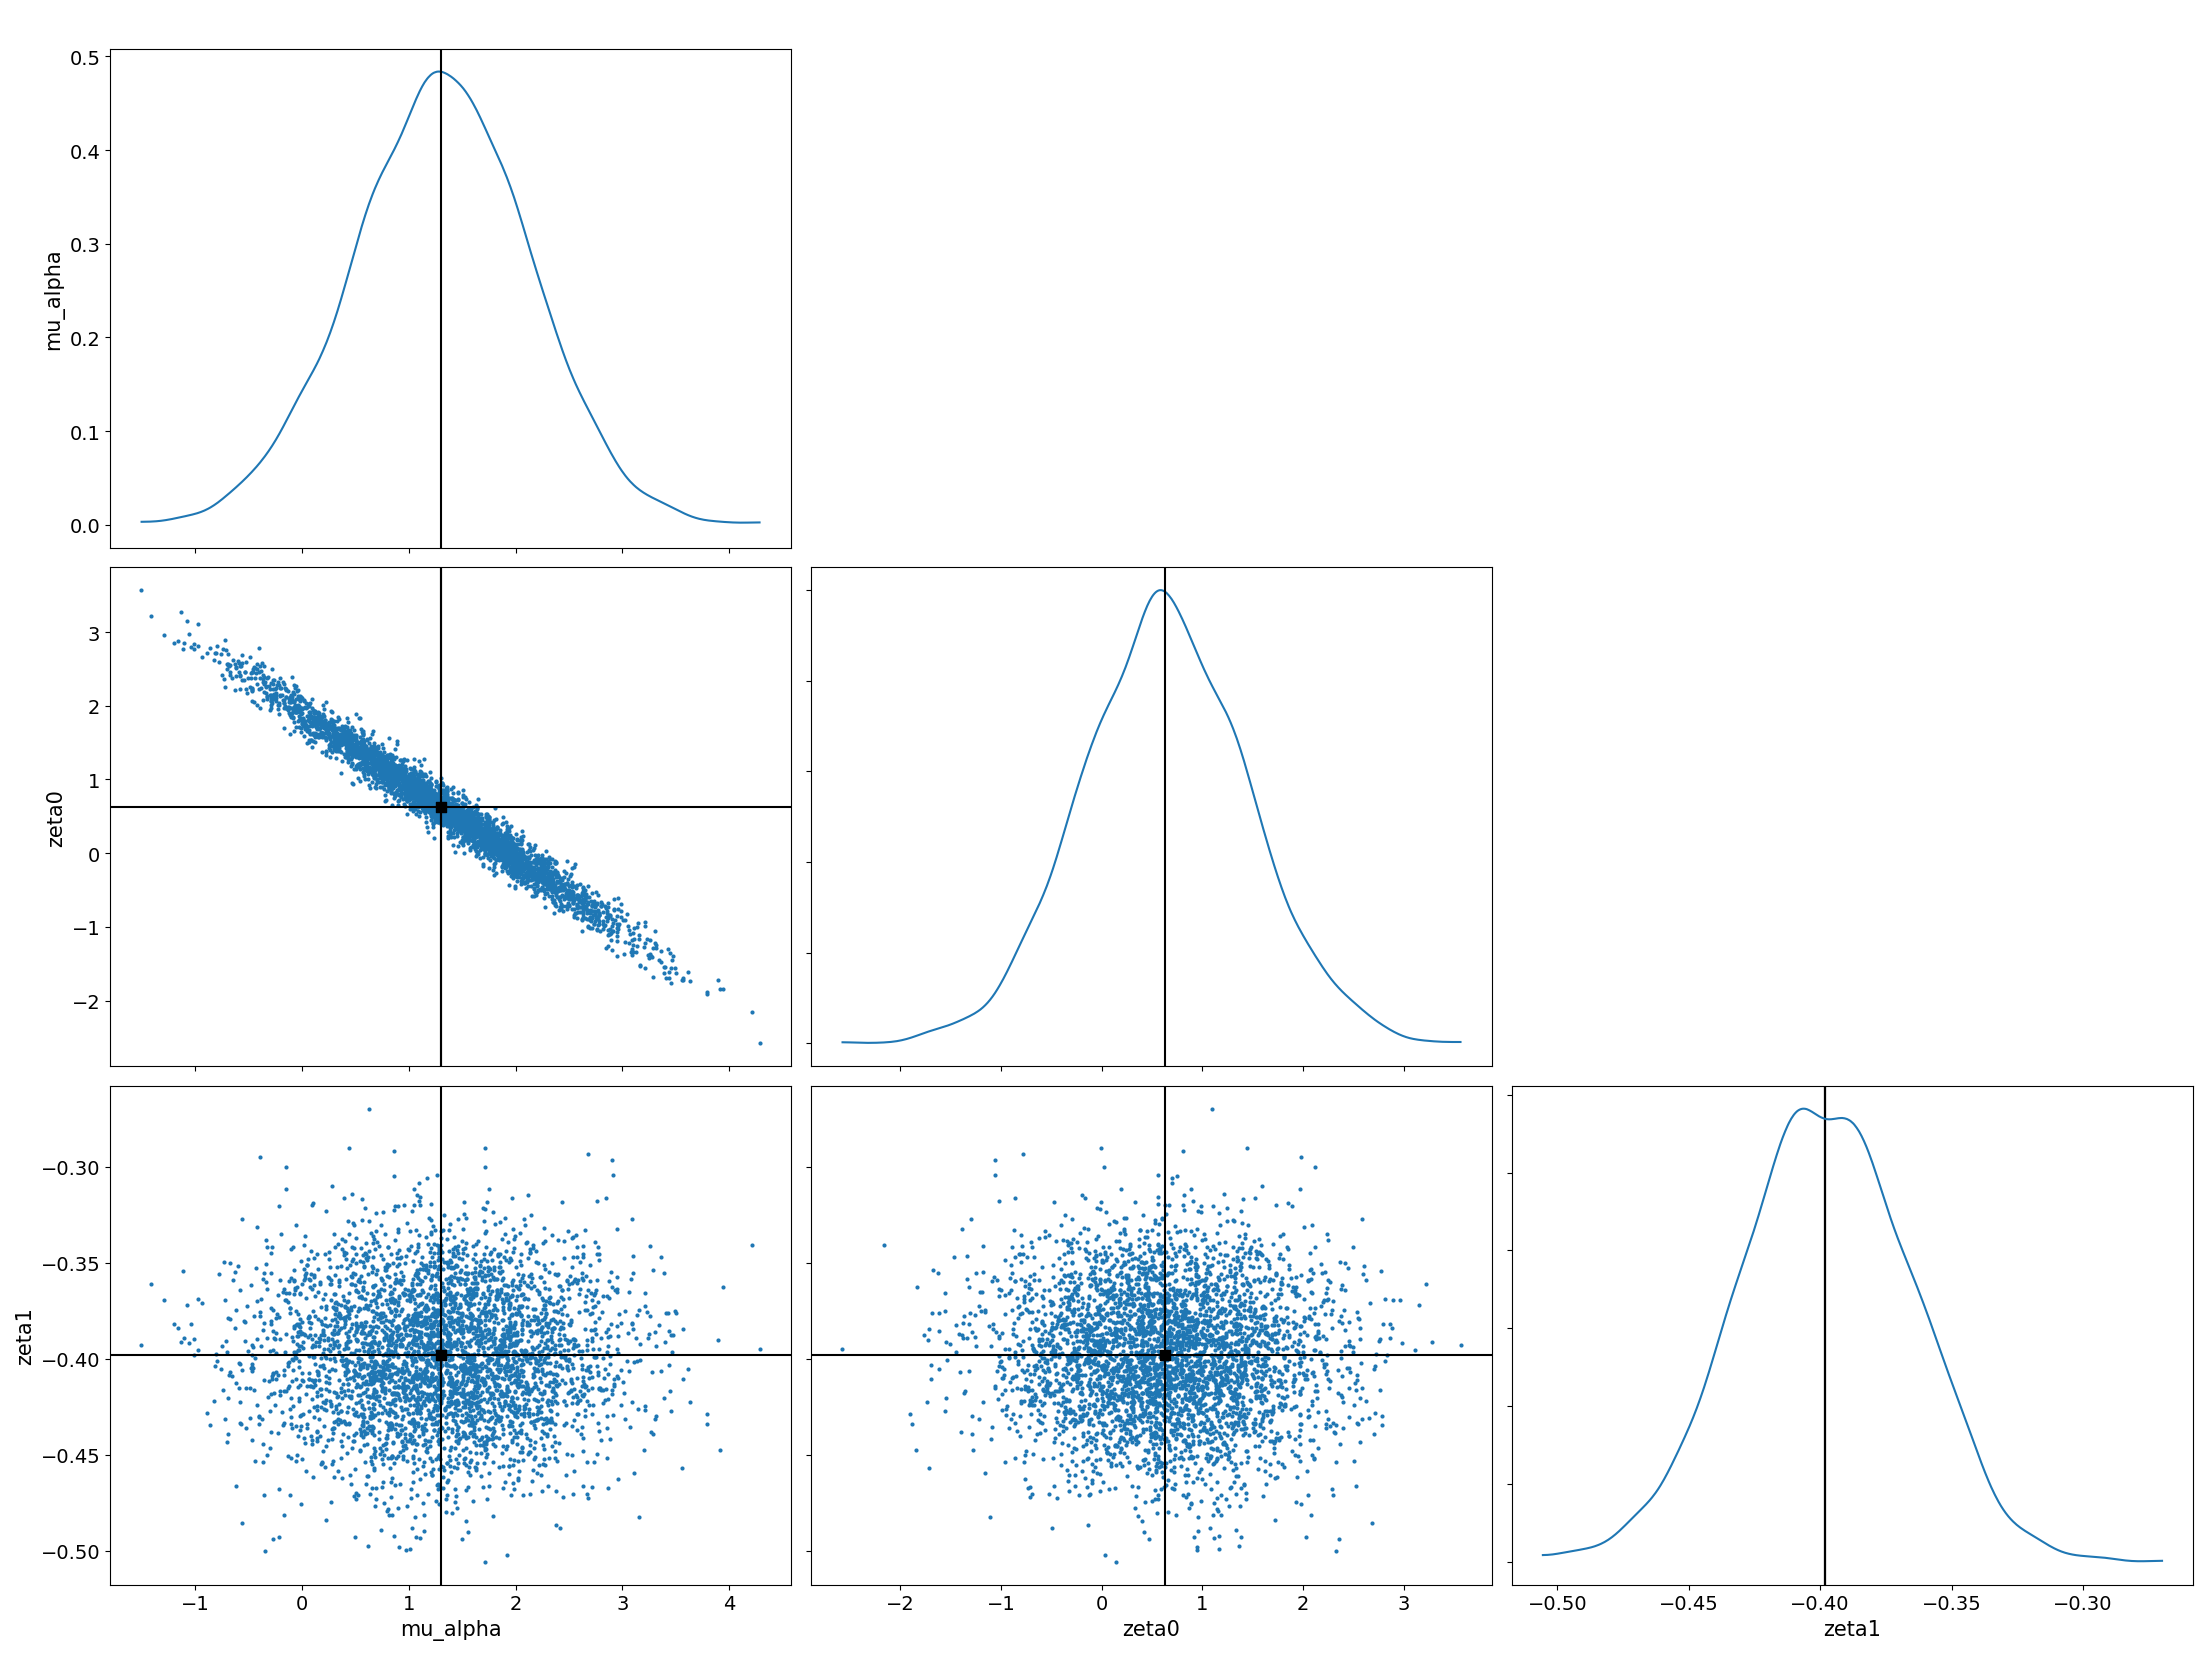
\includegraphics[width=\linewidth]{semiid_sdt_pair.png}
    \caption{Pair plot for $\mu_\alpha$ and $\zeta_0$ from the model with informative prior. The negative correlation ridge persists.}
    \label{fig:semiid_pair}
\end{figure}


\subsection*{Implementation of the Structural Fix: Reparameterization}

The best approach to resolve the structural non-identifiability in this SDT model is reparameterization by removing the condition effect intercept $\zeta_0$.

This adjustment necessitates a change in parameter interpretation. The parameter previously known as $\mu_\alpha$ now represents the average $d'$ when the predictor variable is zero. This parameter is renamed `mu\_alpha\_intercept` to reflect this. The parameter $\zeta\_1$ continues to represent the rate of change in $d'$ with respect to the predictor, now relative to this new baseline.

The modified PyMC code for the identified model is as follows:

\begin{lstlisting}[label=lst:id_sdt_code, caption={PyMC code snippet for the identified SDT model parameters (removing $\zeta_0$).}]
# Priors for Sensitivity (d') parameters
mu_alpha_int = pm.Normal("mu_alpha_int", mu=0.0, sigma=1.0e9) # Was mu_alpha
sigma_alpha = pm.HalfNormal("sigma_alpha", sigma=1.0e9)
# zeta0 = pm.Normal("zeta0", mu=0.0, sigma=1.0e9) # <<< REMOVED
zeta1 = pm.Normal("zeta1", mu=0.0, sigma=1.0e9)

# Person sensitivity intercepts (drawn from mu_alpha_intercept)
alpha_p = pm.Normal("alpha_p", mu=mu_alpha_int, sigma=sigma_alpha)

# Condition Effects on Sensitivity (NO intercept)
gamma_i = pm.Deterministic("gamma_i", zeta1 * cond_pred_data)

# Calculate d' using alpha_p and gamma_i
d_ip = pm.Deterministic("d_ip", alpha_p[...] + gamma_i)

# SDT likelihood calculations are structurally identical
# ...
\end{lstlisting}
By removing the `zeta0` term and defining `gamma\_i` solely based on `zeta1` and the predictor, the additive confounding is eliminated, resulting in a structurally identified model.

\subsection*{Results Following Reparameterization}

If we now fit the reparameterized, identified model using MCMC, we see that the convergence and diagnostics are improved. (Table repeated from before.)

\footnotesize
\begin{verbatim}
--- Identified SDT Model Summary ---
               mean       sd   hdi_3%  hdi_97%  mcse_mean  mcse_sd  ess_bulk  ess_tail  r_hat
mu_alpha_int  1.936    0.149    1.659    2.221      0.008    0.004     380.0     598.0   1.01
zeta1        -0.398    0.033   -0.463   -0.341      0.001    0.000    3558.0    3080.0   1.00
mu_c          0.072    0.062   -0.046    0.186      0.003    0.002     426.0     735.0   1.01
Sampling 4 chains for 1_500 tune and 1_000 draw iterations (6_000 + 4_000 draws total) took 12s.
\end{verbatim}
\normalsize


We see:
\begin{itemize}[label=--, itemsep=1ex]
    \item Good convergence ($\hat{R} \approx 1$) for all parameters.
    \item High Effective Sample Sizes (ESS).
    \item Well-mixed, stable trace plots (in Figure \ref{fig:id_trace}).
\end{itemize}
Following the removal of the confounding source, problematic correlations involving the parameter `mu\_alpha\_intercept` or other model parameters are gone.

Figure \ref{fig:id_pair} shows the pair plot for key parameters from the identified model, including `mu\_alpha\_intercept`. The absence of strong linear correlations shows that the structural non-identifiability has been successfully resolved.

\begin{figure}[tbhp]
    \centering
    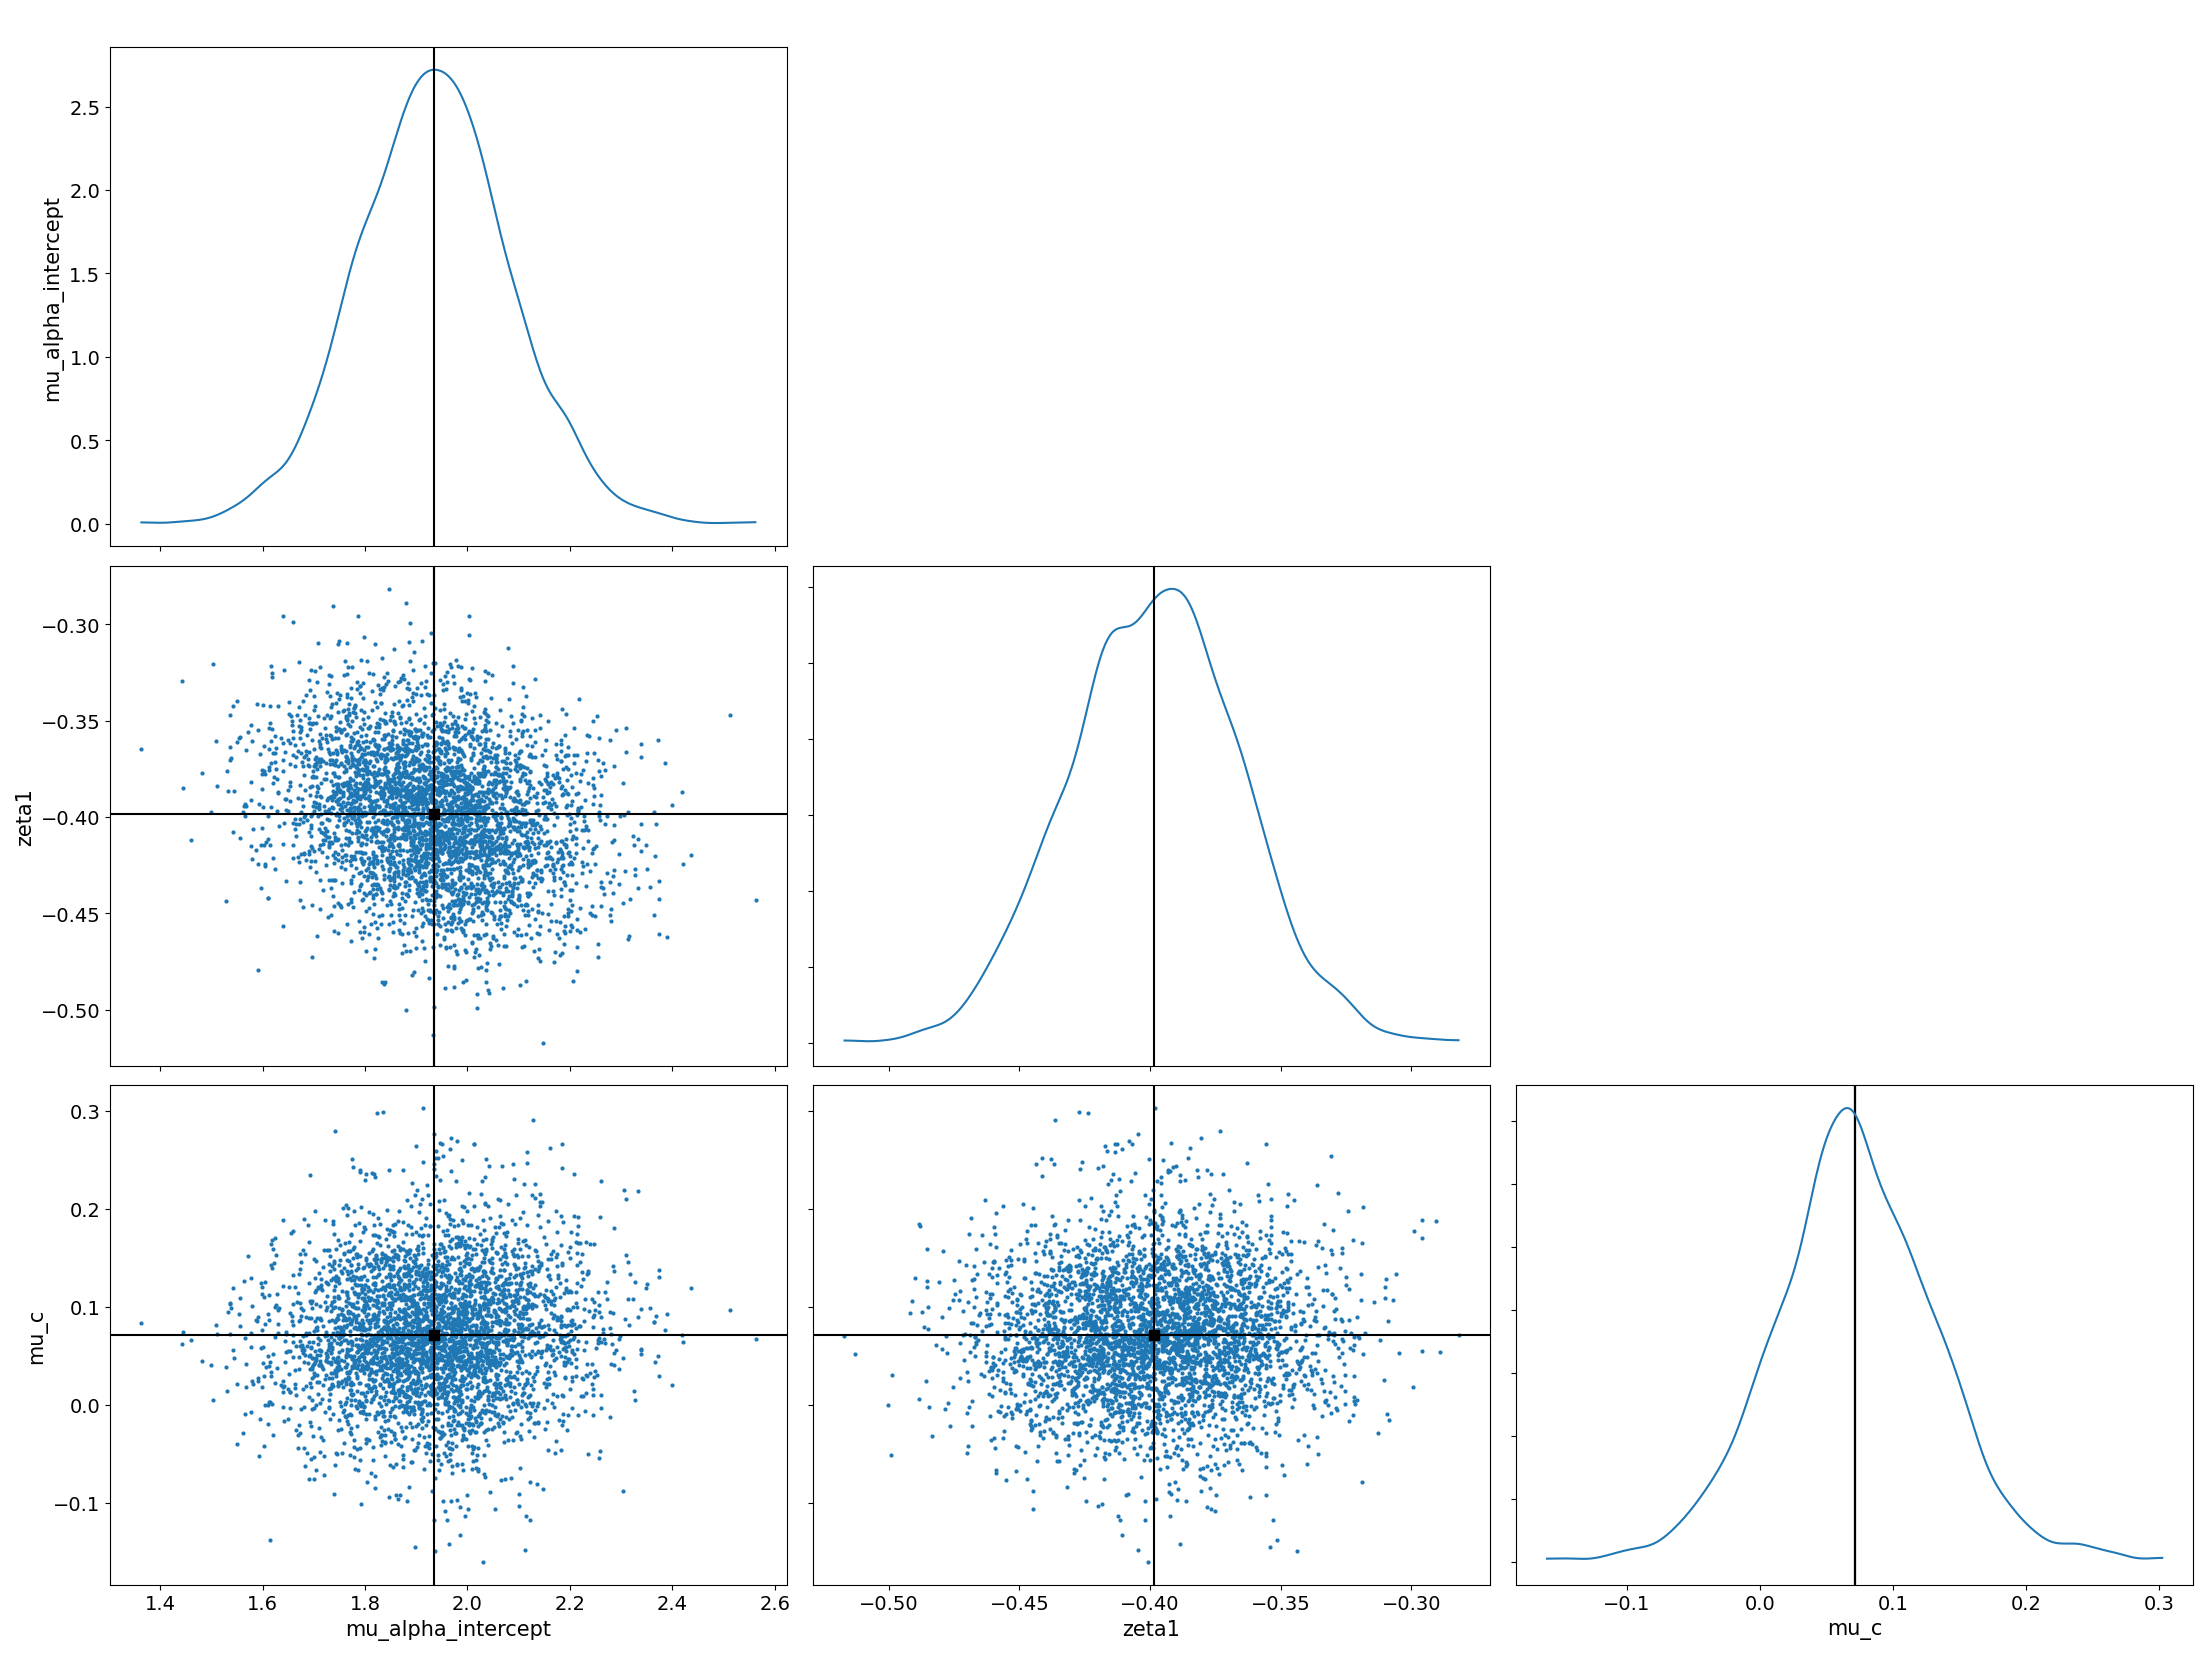
\includegraphics[width=\linewidth]{id_sdt_pair.png}
    \caption{Pair plot for key parameters from the identified SDT model. No strong correlations are evident.}
    \label{fig:id_pair}
\end{figure}


\subsection*{Summary Points}

\begin{itemize}[label=--, itemsep=1ex]
    \item Non-identifiability is a condition where distinct parameter sets produce identical data likelihoods, preventing unique parameter estimation.
    \item In hierarchical models, non-identifiability can arise from redundant parameters, commonly seen with additive intercepts in model components.
    \item The structure $d' = \text{person\_effect} + \text{condition\_effect}$ leads to non-identifiability if both effects incorporate their own intercept terms.
    \item Diagnosis relies on MCMC convergence statistics ($\hat{R}$, ESS) and visual checks such as trace plots and pair plots.
    \item The recommended solution for structural non-identifiability is reparameterization, which removes the underlying redundancy. While informative priors can sometimes assist convergence, they do not fundamentally resolve the structural issue.
    \item It is imperative to assess potential identifiability issues before interpreting model parameters. Models exhibiting convergence problems due to non-identifiability are unlikely to provide reliable inferences regarding the specific parameter values.
\end{itemize}


\end{document}